\usepackage{xcolor}
\usepackage{afterpage}
\usepackage{pifont,mdframed}
\usepackage[bottom]{footmisc}
\usepackage{minted}

\usepackage{tikz}
\usepackage{dsfont}

\createsection{\Grader}{Grader di prova}

\newcommand{\inputfile}{\texttt{stdin}}
\newcommand{\outputfile}{\texttt{stdout}}
\makeatletter
\renewcommand{\this@inputfilename}{\texttt{stdin}}
\renewcommand{\this@outputfilename}{\texttt{stdout}}
\makeatother

Lorenzo e Kevin stanno giocando a Toppabi, una nuova variante del famoso gioco di carte.
Ci sono $5N$ carte, divise in cinque colori: Bianco (\textbf{W}hite), Rosso (\textbf{S}carlet),
Marrone (\textbf{U}mber), Viola (\textbf{P}urple), Smeraldo (\textbf{E}merald). 
Per ogni colore, le carte sono numerate distintamente da $1$ a $N$. Lorenzo pesca $N$ carte, visibili solo a Kevin. 
Toppabi si svolge in due turni. Inizialmente Kevin può utilizzare dei gettoni per dare degli indizi a Lorenzo: con ogni gettone, Kevin 
indica di modificare la posizione di una carta.
Alla fine, Lorenzo posiziona le sue carte. 

\begin{figure}[H]
    \centering
    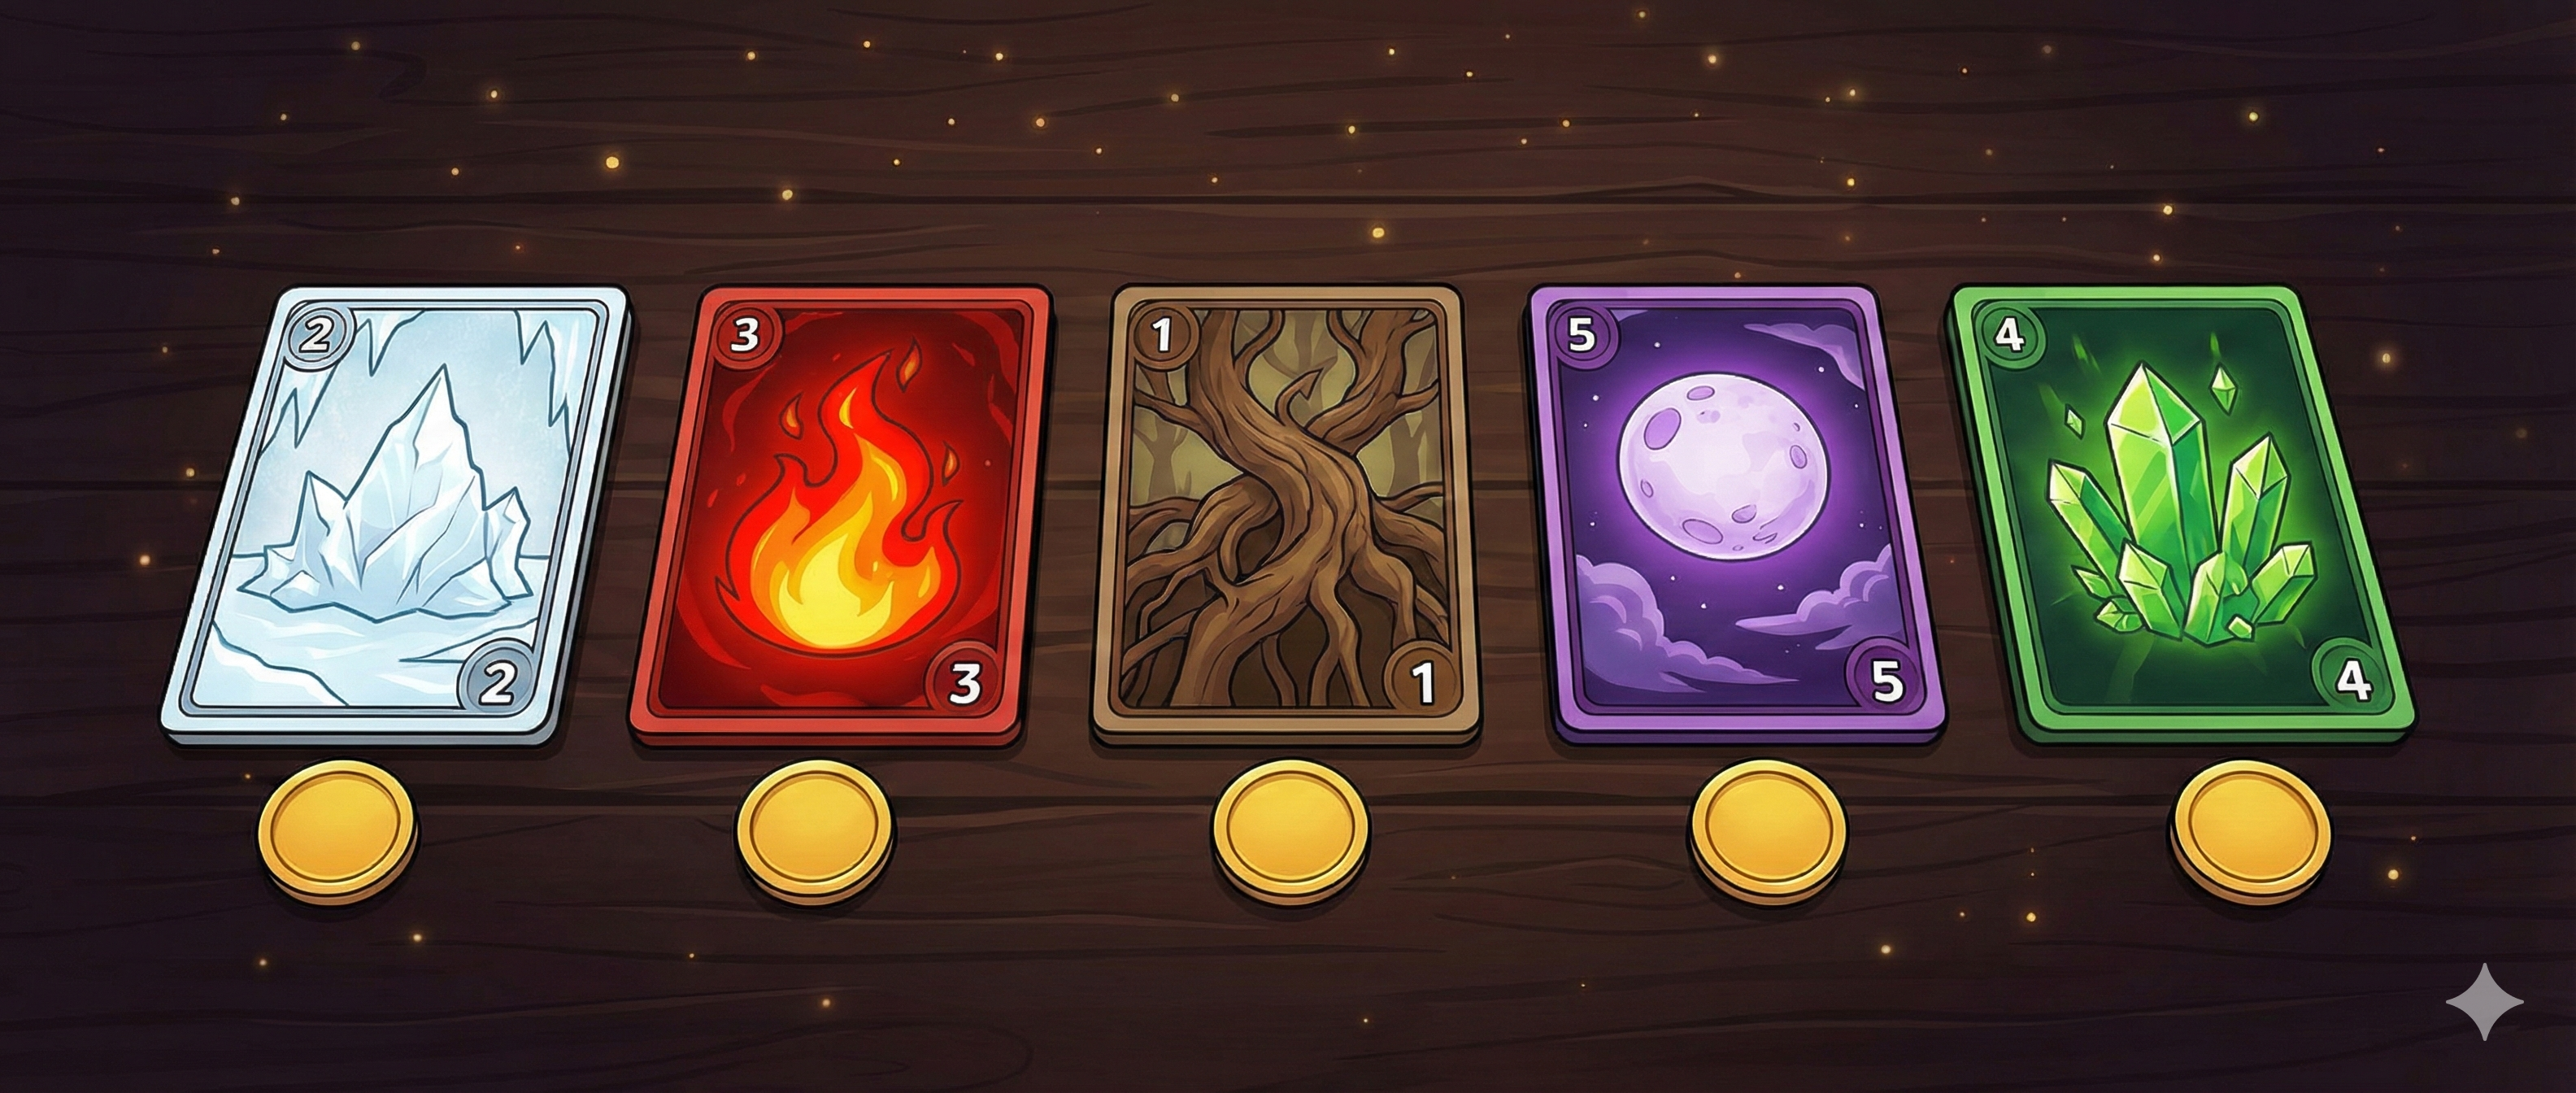
\includegraphics[scale=0.11]{carte2.png}
    \caption{Le carte di Toppabi con i gettoni indizio.}
\end{figure}

Come nel famoso gioco, Lorenzo vuole formare 
fino a cinque mazzetti, dove mazzetto contiene tutte e solo le carte di un colore. Inoltre le carte di un mazzetto devono 
essere ordinate in modo tale che in fondo ci sia la carta con il numero più piccolo e 
in cima quella con il numero più grande. Visto che il verde è il colore preferito di Lorenzo,
vuole che l'ultimo mazzetto contenga le carte di color Smeraldo, se ne possiede qualcuna. 

Kevin quindi decide di utilizzare i gettoni per ordinare le carte di Lorenzo, così che riesca facilmente 
a formare i vari mazzetti nell'ordine corretto. L'ordinamento che Kevin vuole formare è il seguente:
\begin{itemize}
  \item Le carte dello stesso colore devono essere vicine tra di loro.
  \item Le carte dello stesso colore devono essere in ordine crescente.
  \item Le carte di color Smeraldo devono essere tutte a destra.
\end{itemize}
Aiuta Kevin a calcolare il minor numero di gettoni che ha bisogno per ordinare le carte di Lorenzo.

\InputFile
La prima riga contiene un intero $N$, il numero di carte pescate da Lorenzo.

La seconda riga contiene $N$ valori separati da uno spazio, che rappresentano le carte pescate da Lorenzo.
Ogni carta è una stringa composta da un carattere tra $\{\texttt{W}, \texttt{S}, \texttt{U}, \texttt{P}, \texttt{E}\}$,
che rappresenta il colore della carta, seguito un numero intero $V$ tale che $1 \le V \le N$, che rappresenta il numero della carta.

\medskip

\begin{warning}
    Tra gli allegati a questo task troverai un template \texttt{biliardino.*} con un esempio di implementazione.
\end{warning}

\OutputFile
Stampa un singolo intero, il numero minimo di gettoni necessari a Kevin per ordinare le carte di Lorenzo secondo le regole descritte.

\Constraints
\begin{itemize}
    \item $1 \le N \le 100\,000$.
    \item Le carte pescate da Lorenzo sono tutte distinte.
\end{itemize}

\Scoring
\begin{itemize}
  \item \subtask Casi d'esempio.
  \item \subtask Per ogni colore c'è una sola carta.
  \item \subtask Per ogni colore ci sono al massimo due carte e i colori sono ordinati tra loro secondo 
    $\texttt{W} \prec \texttt{S} \prec \texttt{U} \prec \texttt{P} \prec \texttt{E}$.
  \item \subtask Tutte le carte sono di colore $\texttt{W}$, $N \le 2\,000$. 
  \item \subtask $N \le 2\,000$.
  \item \subtask Nessuna limitazione aggiuntiva.
\end{itemize}

\Examples

\begin{example}
    \exmpfile{input0.txt}{output0.txt}
    \exmpfile{input1.txt}{output1.txt}
\end{example}

\Explanations

Nel \textbf{primo caso d'esempio}, Kevin può utilizzare un gettone per spostare la carta \texttt{E1} all'ultima posizione e 
un altro gettone per spostare la carta \texttt{P1} alla prima posizione.

Nel \textbf{secondo caso d'esempio}, le carte sono già ordinate secondo le regole di Kevin.